\apendice{Documentación}

\section{Introducción}
En esta parte de la documentación se encuentra el manual de usuario, que será de utilidad para
el uso de la aplicación por parte de cualquier usuario. En él se enseña tanto a entrar en la aplicación a través de la máquina virtual, como de usar la aplicación en su totalidad.

\section{Manual de usuario}

\subsection{Acceder a la web}
Para acceder a la web, se puede hacer de dos formas:
\begin{itemize}
    \tightlist
    \item Si estamos utilizando el entorno virtual, el acceso es a través de cualquier navegador, introduciendo la dirección ``http://localhost:81''.
    \item Si estamos utilizando y lanzando la aplicación desde Visual Studio, al compilar y ejecutar nos carga la web directamente en el navegador que esté configurado (este se puede modificar desde el lanzador de Visual Studio).
\end{itemize}

\subsection{Inicio de sesión}
Una vez ejecutamos la aplicación, la primera pantalla que veremos es la de iniciar sesión.

\begin{figure}
    \centering
    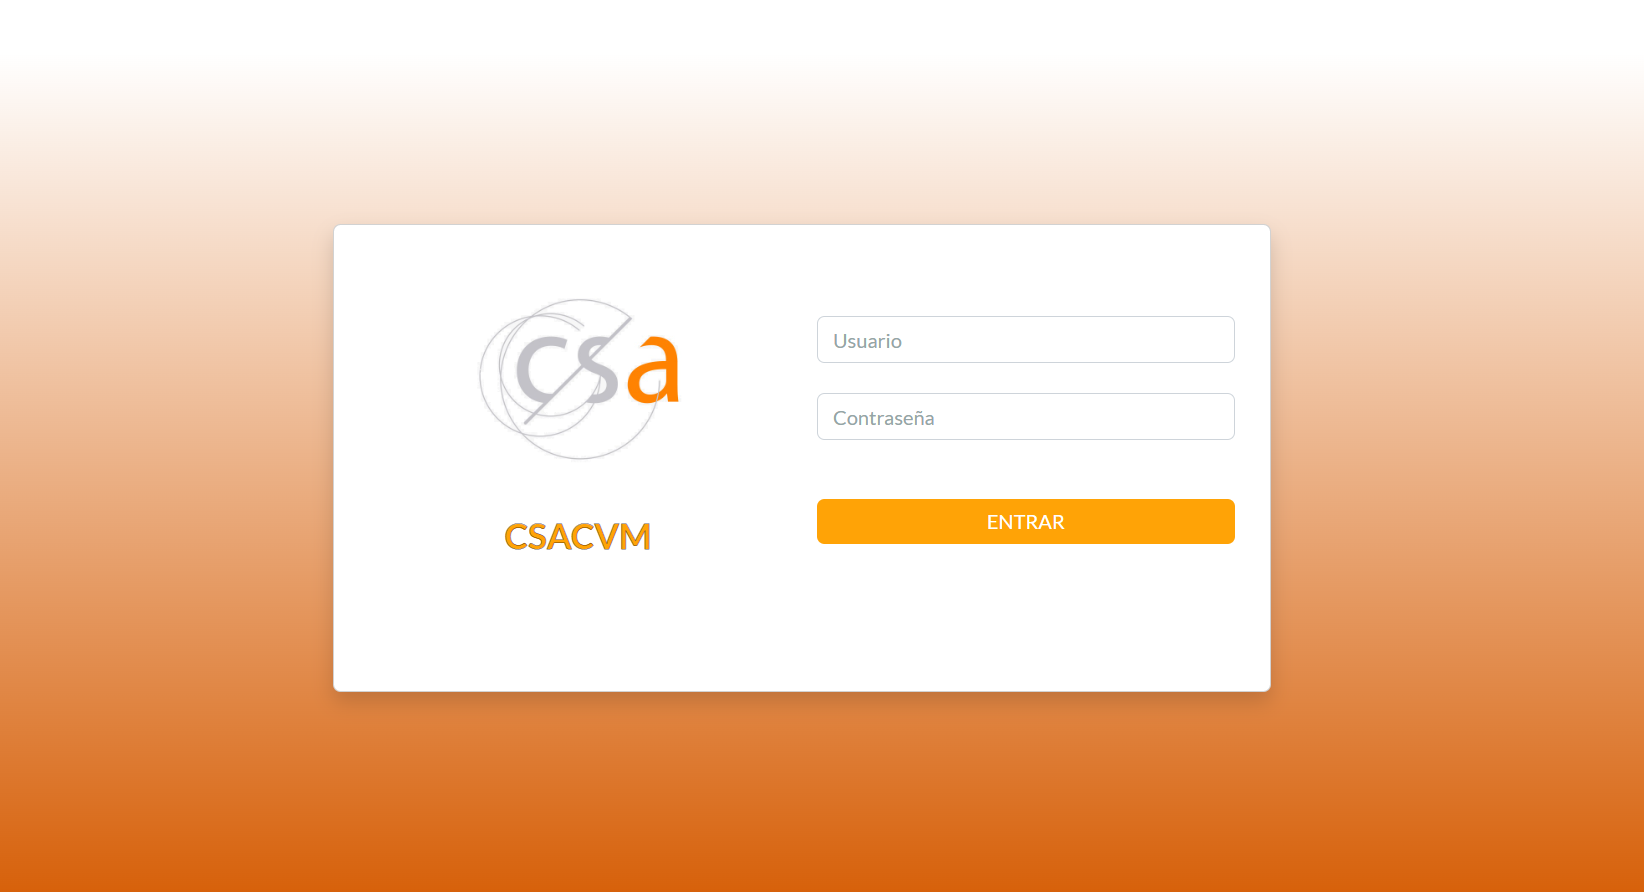
\includegraphics[width=\linewidth]{img/ManualUsuario/Manual01.png}
    \caption{Manual CSACVM - Inicio de sesión}
\end{figure}

Para entrar en la aplicación, debemos utilizar un usuario que esté registrado. Los usuarios se pueden crear a través de un administrador, pero actualmente, hay dos usuarios de prueba:
\begin{itemize}
    \tightlist
    \item Admin: admin.admin, contraseña = 1234.
    \item Usuario normal: userPrueba, contraseña = 2022.
\end{itemize}

Si la validación es correcta, se nos permitirá el acceso a la aplicación. 

\subsection{Página principal}
Una vez dentro de la aplicación, la pantalla principal tendrá el aspecto de la figura \ref{manualIndex}

\begin{figure}
    \centering
    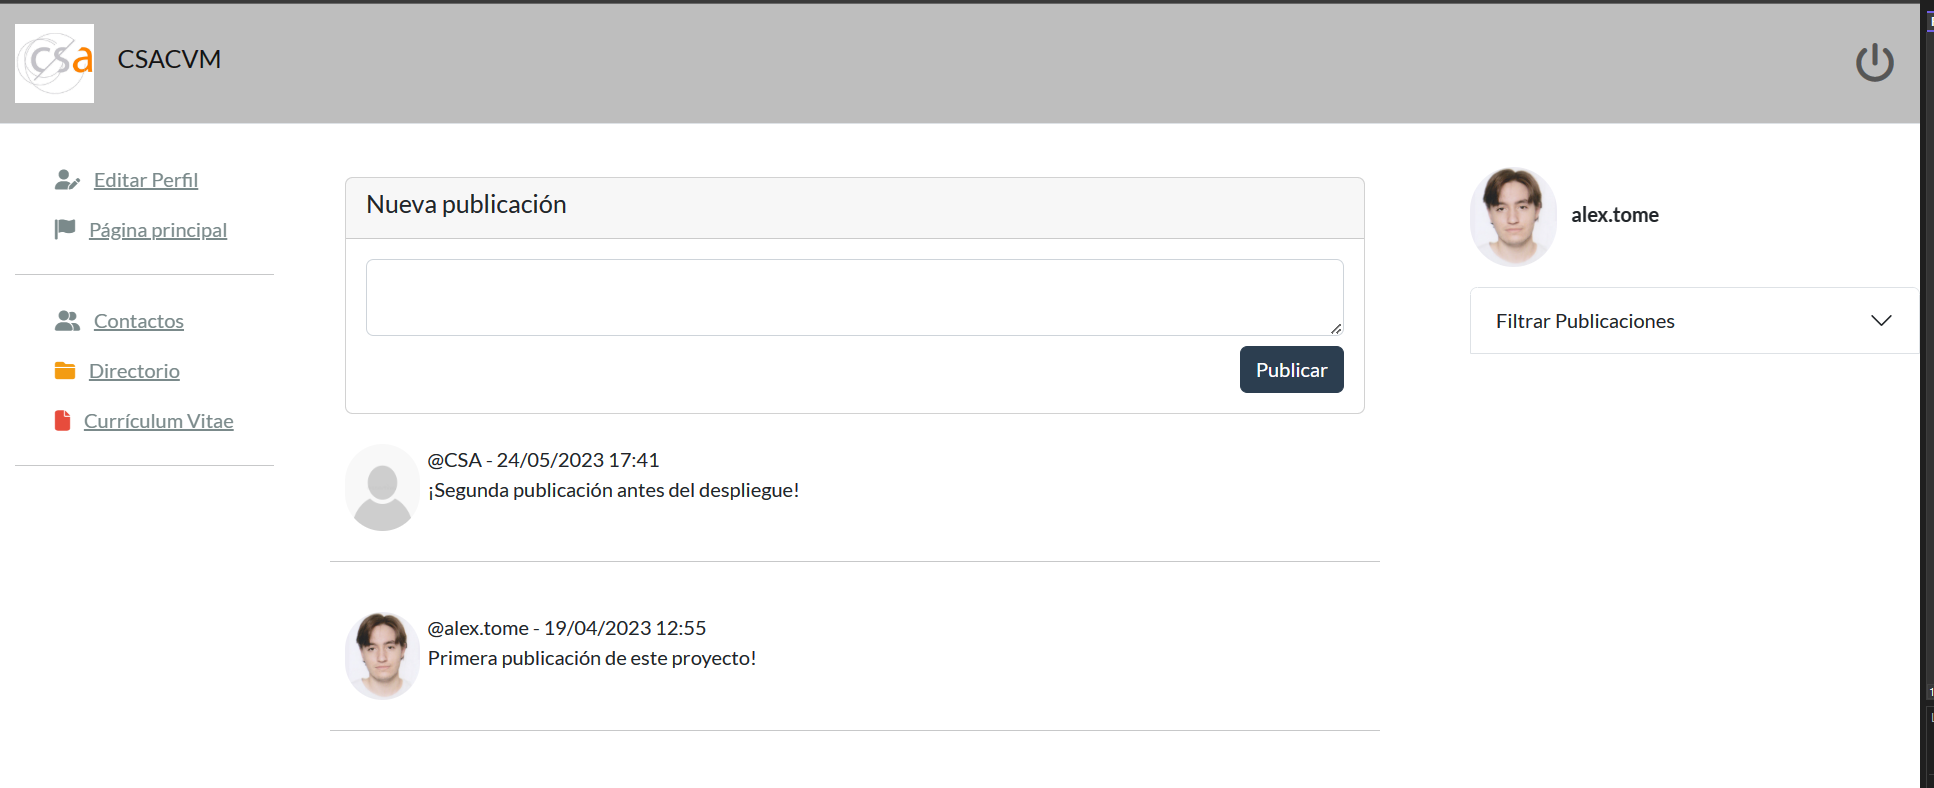
\includegraphics[width=\linewidth]{img/ManualUsuario/Manual02.png}
    \caption{Manual CSACVM - Layout y página principal} 
    \label{manualIndex}
\end{figure}

\begin{figure}
    \centering
    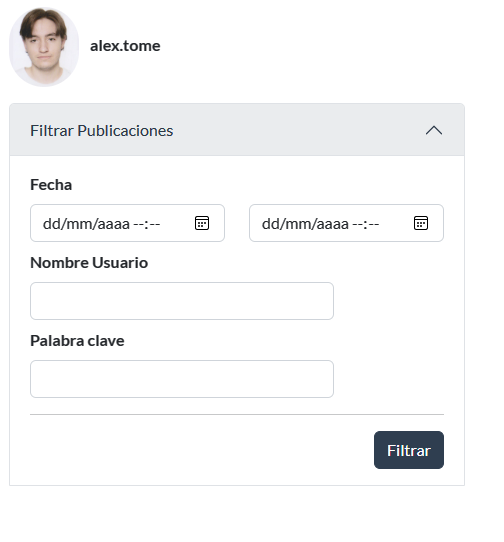
\includegraphics[width=.9\linewidth]{img/ManualUsuario/Manual03.png}
    \caption{Manual CSACVM - Filtros publicaciones} 
\end{figure}

En dicha pantalla podemos distinguir tres zonas distintas. A la izquierda, una barra con las distintas opciones para cada usuario, en el centro, las publicaciones de la aplicación y una zona para escribir un nuevo ``post'', y a la derecha, los filtros para la visualización de las publicaciones.

En los filtros de las publicaciones, podemos indicar el intervalo de fechas, el nombre de usuario o alguna palabra clave.

En el panel lateral izquierdo, las opciones dependerán del usuario con el que se haya iniciado sesión, tal y como se ve en la figura \ref{manualLayout}. 
\begin{figure}
    \centering
        \subfloat[Opciones no administrador]{
        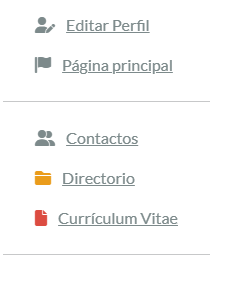
\includegraphics[width=0.4\textwidth]{img/ManualUsuario/Manual09.png}}
        \subfloat[Opciones administrador]{
        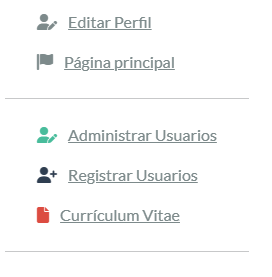
\includegraphics[width=0.4\textwidth]{img/ManualUsuario/Manual10.png}}
    \caption{Manual CSACVM - Panel lateral opciones}
    \label{manualLayout}
\end{figure}

Como vemos en la figura \ref{manualLayout}, dependiendo de si el usuario es administrador o no, nos saldrán unas opciones u otras, aunque haya varias que compartan ambos. Además, la vista de currículos también es distinta en cada caso.


\subsection{Perfil de usuario}
Si le damos en editar perfil, se nos mostrará nuestro perfil de usuario.
\begin{figure}
    \centering
    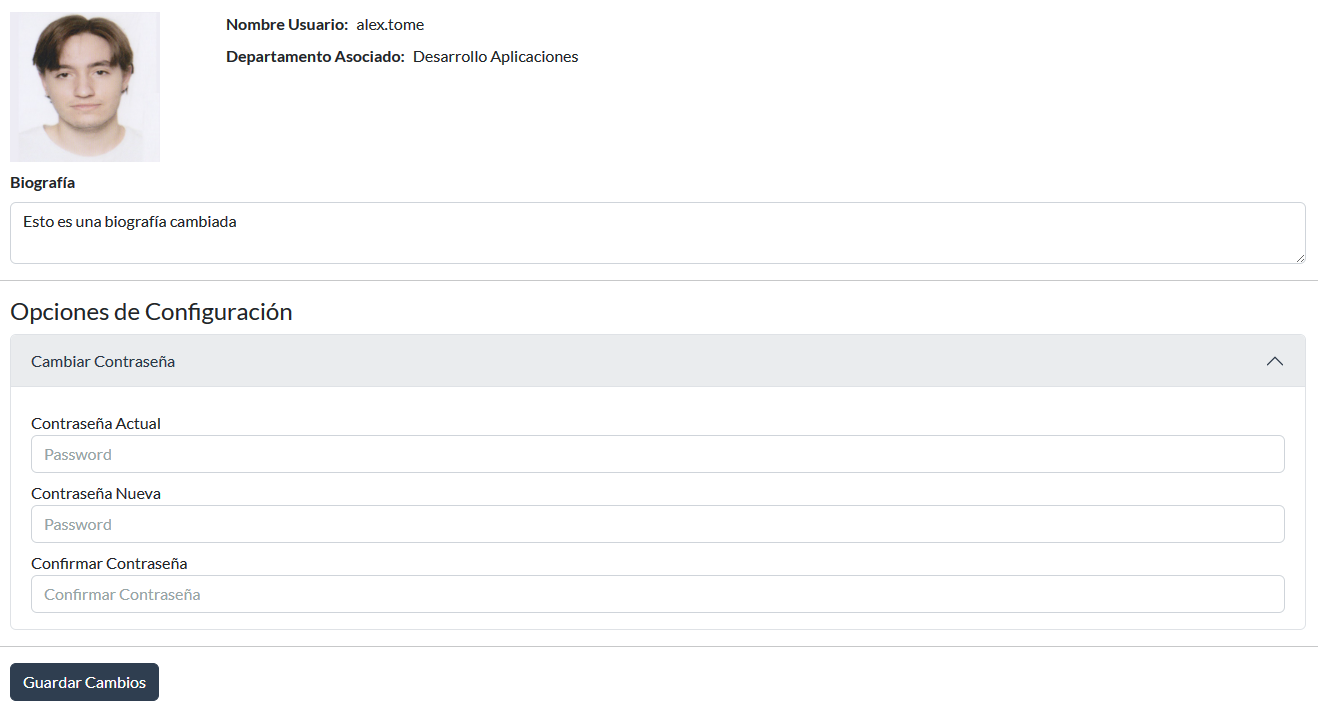
\includegraphics[width=\linewidth]{img/ManualUsuario/Manual04.png}
    \caption{Manual CSACVM - Perfil de usuario}
    \label{manualPerfil}
\end{figure}

En este apartado (fig. \ref{manualPerfil}), podremos hacer lo siguiente:
\begin{itemize}
    \item Cambiar la foto de perfil: al hacer click sobre la imagen, podemos subir una imagen desde nuestro directorio y cambiarla.
    \item Cambiar la biografía: al igual que cualquier red social, se permite añadir una biografía a modo de descripción del usuario.
    \item Cambiar contraseña: opción para cambiar la contraseña con la que entramos a la aplicación.
\end{itemize}

Para guardar los cambios, solo tenemos que pulsar al botón inferior.

\subsection{Contactos}
En el apartado de contactos, podemos buscar usuarios registrados en la aplicación y añadirlos como usuarios favoritos, similar a la funcionalidad que tiene skype.
\begin{figure}
    \centering
    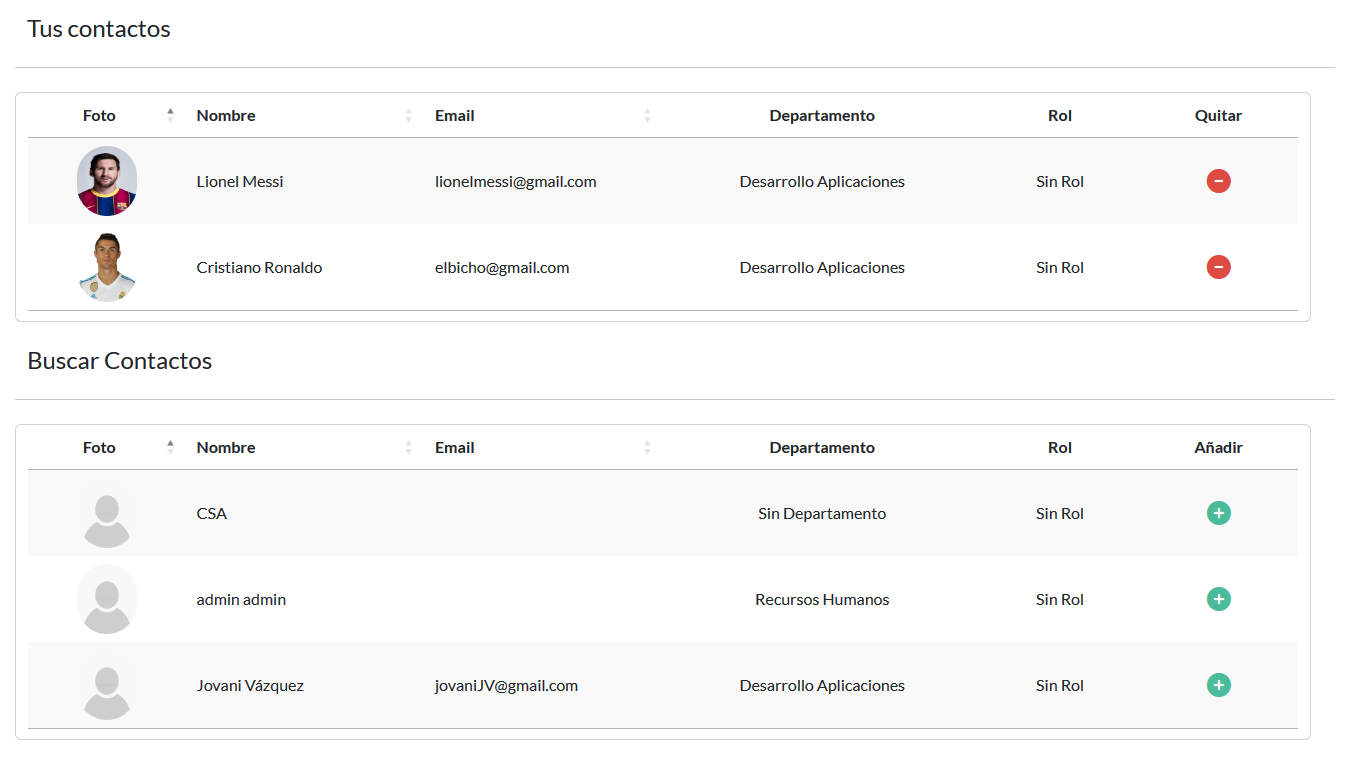
\includegraphics[width=\linewidth]{img/ManualUsuario/Manual05.png}
    \caption{Manual CSACVM - Contactos}
    
\end{figure}

De momento la funcionalidad es sencilla, en la tabla superior tenemos nuestros contactos, los cuales podemos quitar, y en la tabla inferior al revés.


\subsection{Directorio y notas}
En el directorio de usuario podemos crear notas. A través del botón superior, podemos darle título y contenido a una nota, la cual podremos ver, modificar o eliminar.
\begin{figure}
    \centering
    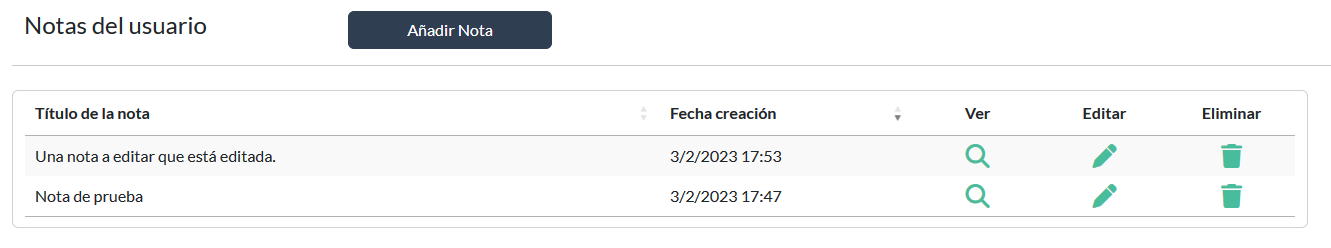
\includegraphics[width=\linewidth]{img/ManualUsuario/Manual06.png}
    \caption{Manual CSACVM - Directorio}  
\end{figure}

Para crear una nota, se nos abre la vista de la figura \ref{manualNotas}
\begin{figure}
    \centering
    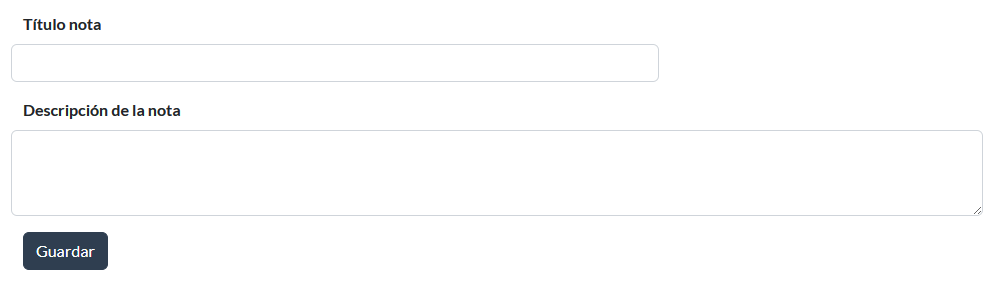
\includegraphics[width=\linewidth]{img/ManualUsuario/Manual07.png}
    \caption{Manual CSACVM - Crear notas}
    \label{manualNotas}
\end{figure}

De esta forma podemos añadir un título que describirá el contexto de la nota y es lo que visualizaremos en la tabla, así como el contenido de la nota en sí.

\subsection{Currículum}
La vista de los currículos y la funcionalidad de cada uno de los apartados será distinta para cada tipo de usuario.
\subsubsection{Currículos para usuarios genéricos}
\begin{figure}
    \centering
    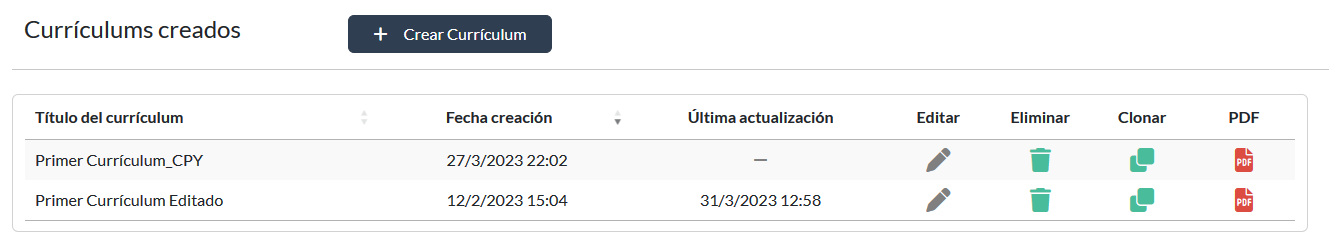
\includegraphics[width=\linewidth]{img/ManualUsuario/Manual11.png}
    \caption{Manual CSACVM - Currículos para no administradores}
    
\end{figure}

Esta es la vista para usuarios genéricos. La tabla contiene los currículos creados por el usuario que se encuentra en la aplicación. Para crear un nuevo currículum, solo tenemos que hacer click en el botón superior, e insertar el título del currículum.

También tenemos la opción de clonar a partir de otro currículum, de forma que se hará una copia de los datos de ese currículum a uno nuevo.

Una vez creado, tenemos las siguientes posibilidades:
\begin{itemize}
    \item \textbf{Editar}: es la funcionalidad principal, al hacer click en este botón, accederemos a una vista en la que tendremos las distintas opciones para rellenar el currículum.
    \item \textbf{Eliminar}: se hace un borrado completo del currículum.
    \item \textbf{PDF}: se hace una exportación del currículum a formato PDF.
\end{itemize}

Al hacer click en editar currículum, se nos mostrará la vista de la figura \ref{manualEditar}. Dentro de la vista tenemos varias etapas a rellenar:
\begin{figure}
    \centering
    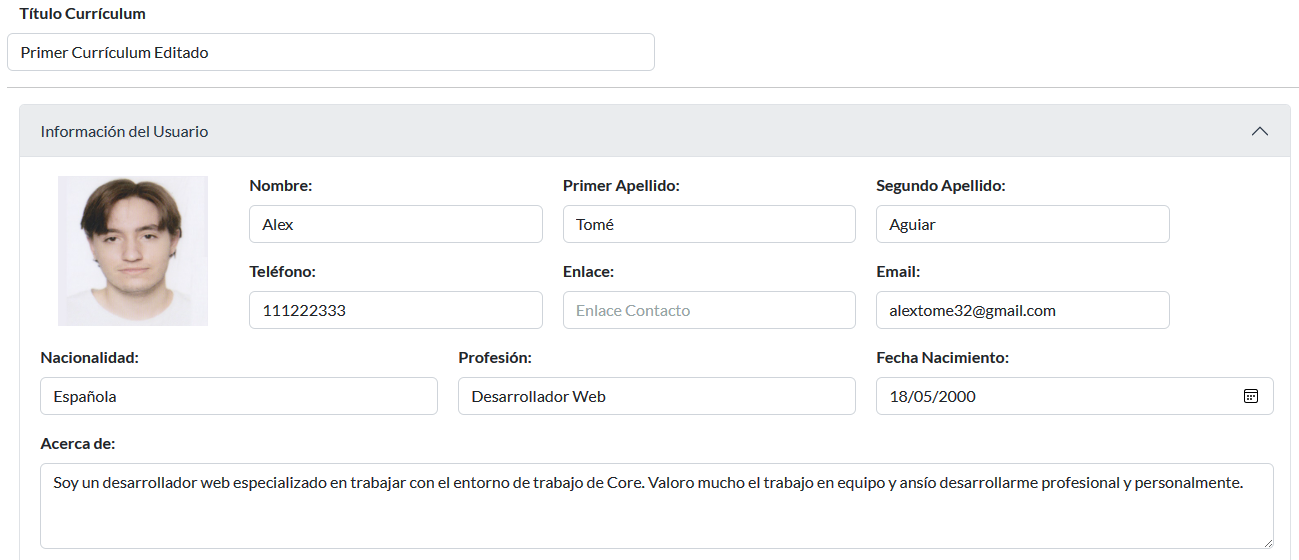
\includegraphics[width=\linewidth]{img/ManualUsuario/Manual12.png}
    \caption{Manual CSACVM - Editar currículum}
    \label{manualEditar}
\end{figure}

\begin{itemize}
    \item \textbf{Información del usuario}: datos principales del usuario.
    \item \textbf{Formación Académica}: estudios del usuario.
    \item \textbf{Idiomas}: si se ha obtenido un título de un idioma.
    \item \textbf{Experiencia laboral}: los diferentes empleos que ha tenido el usuario.
    \item \textbf{Aptitudes y logros}: a modo de añadir información de carácter personal.
\end{itemize}


\begin{figure}
    \centering
    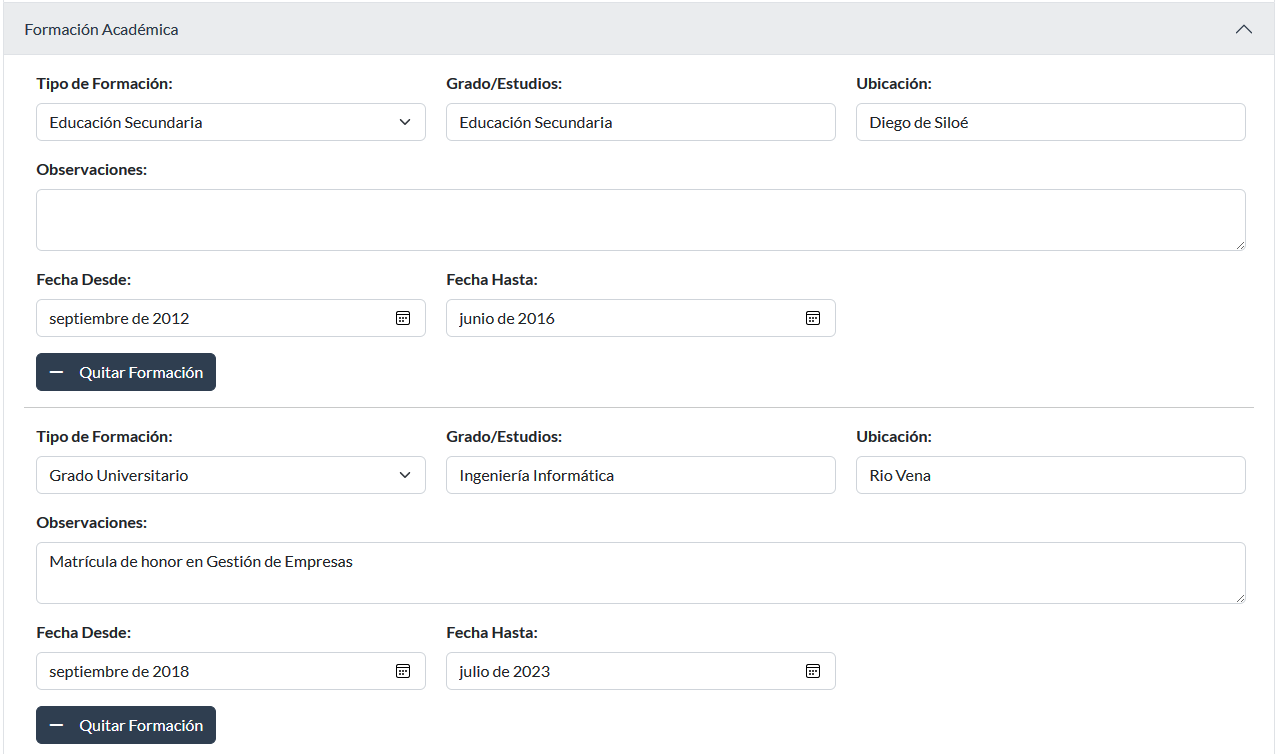
\includegraphics[width=\linewidth]{img/ManualUsuario/Manual13.png}
    \caption{Manual CSACVM - Editar currículum: formación académica}
    
\end{figure}

En este apartado podemos añadir tantas entradas como queramos, al igual que en los siguientes. 

En la formación podemos indicar el tipo de formación, qué estudios se han realizado, dónde y un campo de observaciones opcional de carácter informativo. 

Además de eso se indica cuándo se realizó.

\begin{figure}
    \centering
    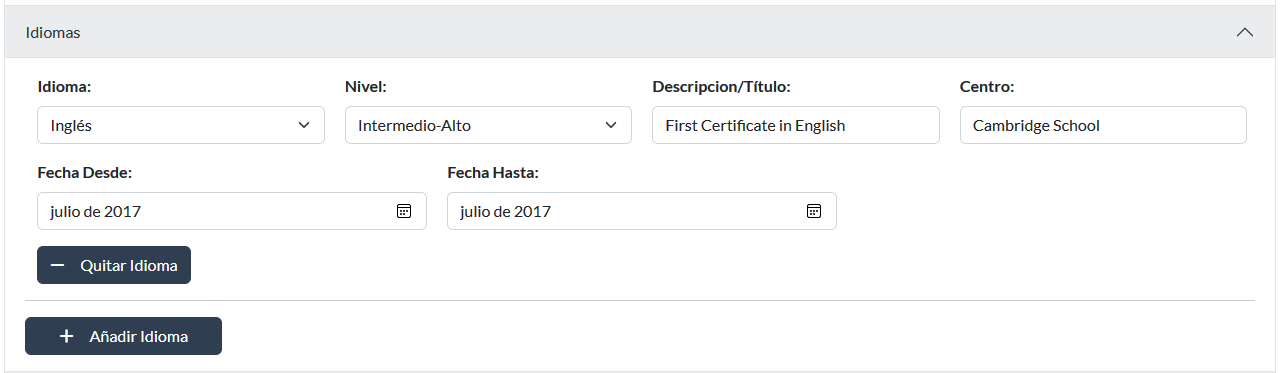
\includegraphics[width=\linewidth]{img/ManualUsuario/Manual14.png}
    \caption{Manual CSACVM - Editar currículum: Idiomas} 
\end{figure}
En la parte de los idiomas, nos permite elegir el idioma, el nivel, la descripción o el título que se ha obtenido y dónde se realiza, además de indicar cuándo se realizó o se obtuvo el título.

\begin{figure}
    \centering
    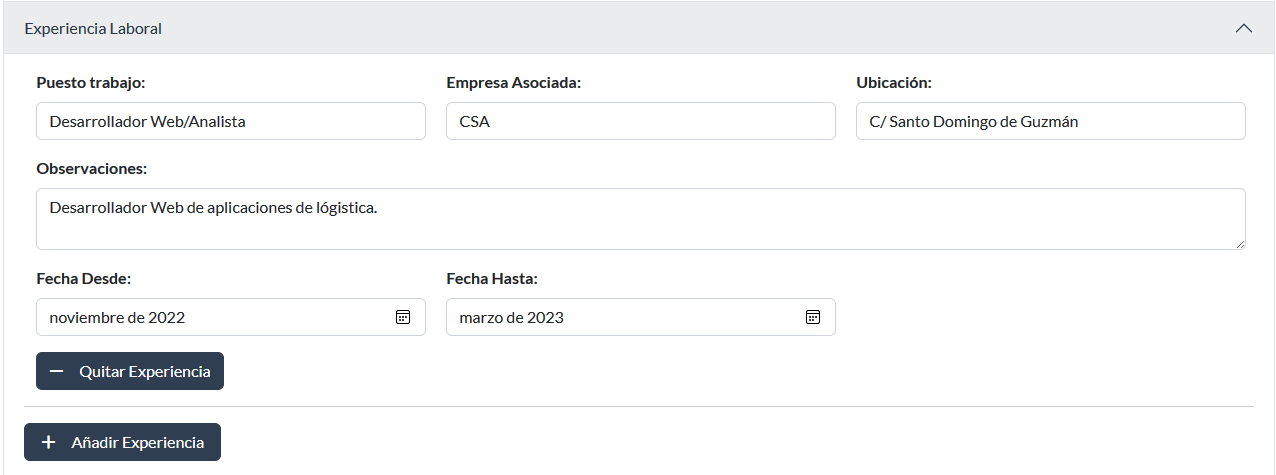
\includegraphics[width=\linewidth]{img/ManualUsuario/Manual15.png}
    \caption{Manual CSACVM - Editar currículum: Experiencia laboral}
\end{figure}
En el apartado de la experiencia laboral se debe indicar el puesto principal de trabajo, la empresa en la que se realizó y su ubicación (esto último opcional), y un campo de observaciones para añadir más información sobre el puesto de trabajo, así como los años que se estuvo trabajando.

 
\begin{figure}
    \centering
    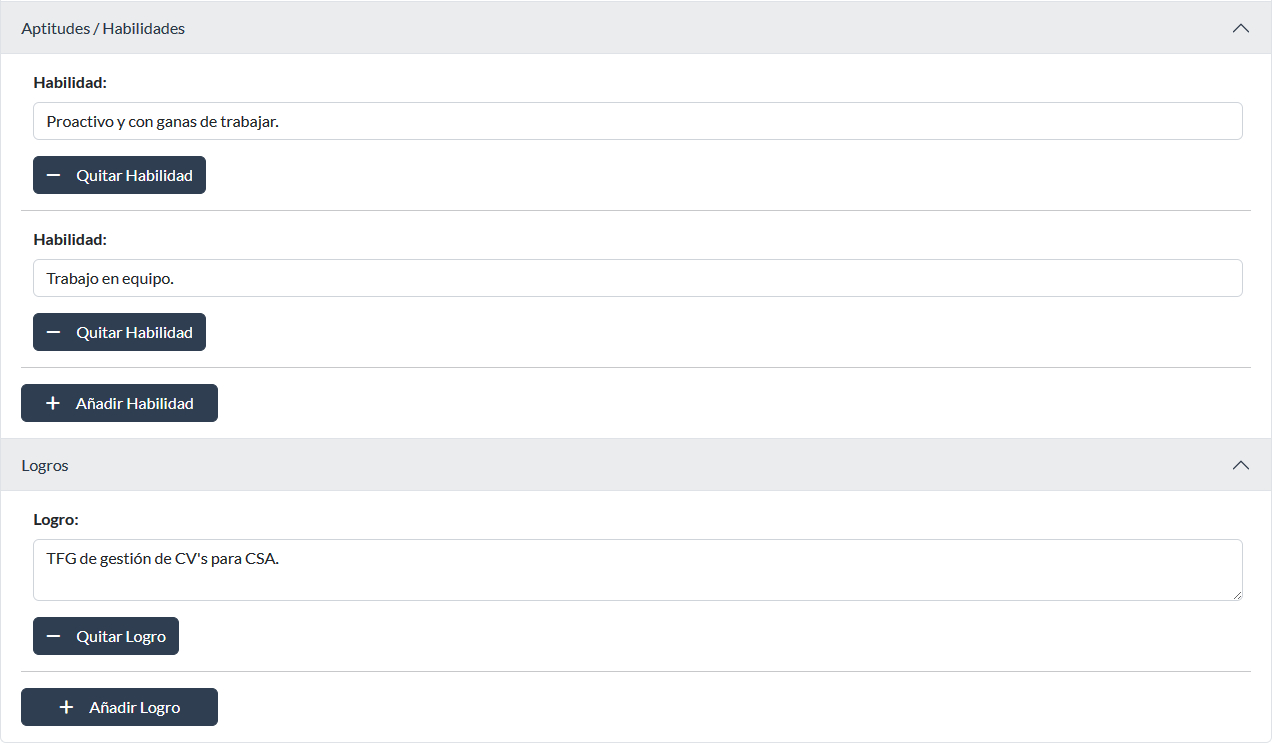
\includegraphics[width=\linewidth]{img/ManualUsuario/Manual16.png}
    \caption{Manual CSACVM - Editar currículum: Aptitudes y Logros} 
    \label{manualLogros}
\end{figure}
Finalmente tenemos los apartados de aptitudes y logros (fig. \ref{manualLogros}), que añaden información auxiliar para completar el currículum. Estos apartados son de carácter personal, en los que se indican atributos del trabajador como modelo de trabajo, personalidad, carácter, etc.

\subsubsection{Exportación a PDF}
\begin{figure}
    \centering
    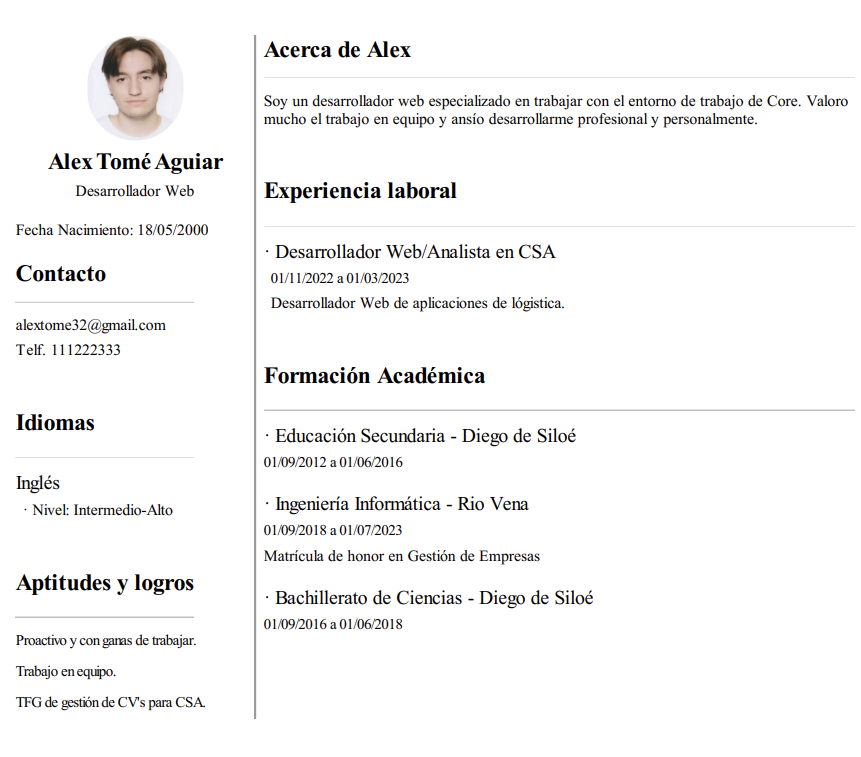
\includegraphics[width=\linewidth]{img/ManualUsuario/Manual17.png}
    \caption{Manual CSACVM - Exportación PDF}
    \label{manualPDF}
\end{figure}
Los PDF's tienen el formato europeo de currículos (fig. \ref{manualPDF}), de modo que se encuentran, por un lado, la foto y los datos principales y más personales del usuario a la izquierda, y por otro, la experiencia laboral y la formación académica a la derecha (junto con el acerca de).

Al hacer un formato específico y estandarizado, todos los usuarios de la aplicación tendrán el mismo tipo de PDF y será más fácil para extraer datos y organizarlos por parte de la administración de la empresa.

\subsection{Currículum de administradores}
La vista de currículos para administradores es algo distinta (fig. \ref{manualCNA}). En primer lugar, los currículos que se ven en la tabla son todos los que están en el sistema de los diferentes usuarios.

\begin{figure}
    \centering
    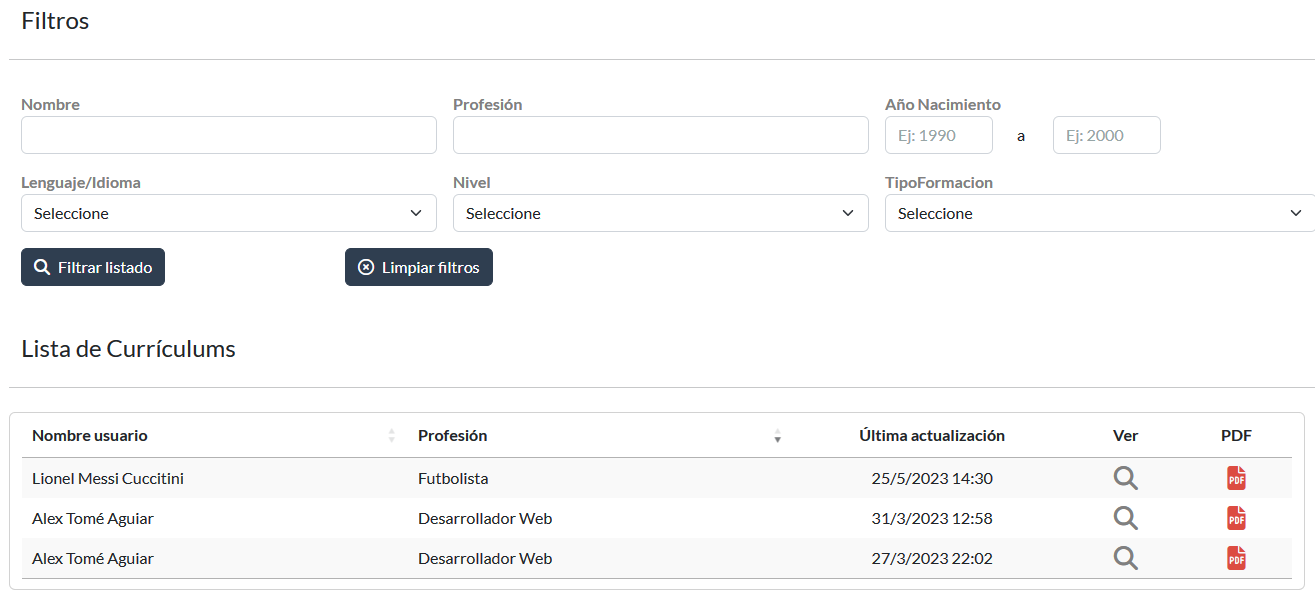
\includegraphics[width=\linewidth]{img/ManualUsuario/Manual19.png}
    \caption{Manual CSACVM - Currículos para administradores}
    \label{manualCNA}
\end{figure}
En la parte superior tenemos los filtros, por los que podemos buscar los currículos en profundidad a través de los campos que queramos (idiomas, año nacimiento del usuario, nombre...). 

En la parte inferior tenemos la tabla con todos los currículos del sistema. Dentro podremos ver el contenido de los currículos o imprimirlos.

\begin{figure}
    \centering
    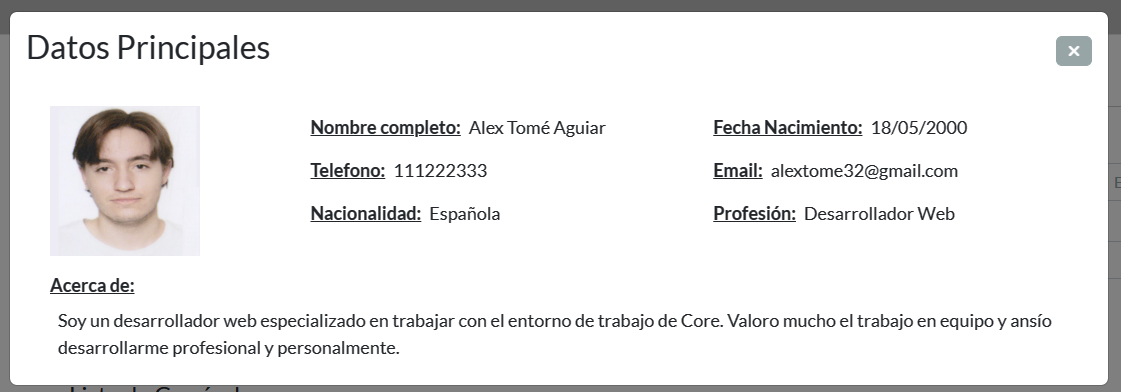
\includegraphics[width=\linewidth]{img/ManualUsuario/Manual20.png}
    \caption{Manual CSACVM - Ver currículum}  
\end{figure}

\subsection{Registro de usuarios}
\begin{figure}
    \centering
    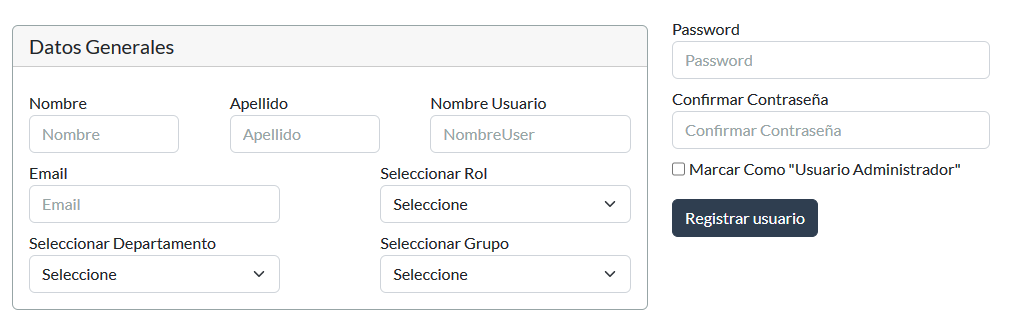
\includegraphics[width=\linewidth]{img/ManualUsuario/Manual21.png}
    \caption{Manual CSACVM - Registro de usuarios}
    \label{manualRegistro}
\end{figure}
En la pantalla del registro de usuarios (fig. \ref{manualRegistro}), un administrador podrá añadir un usuario al sistema.
Para ello, debe completar los diferentes campos que se marcan. 

Hay varios de ellos que son obligatorios, como por ejemplo el nombre de usuario o la contraseña, que son con los que podrá entrar a la aplicación. Después tenemos campos opcionales como el email, el nombre y apellido, el departamento, el rol o el grupo.

Además de esto, podemos indicar si el usuario es administrador o no.

\subsection{Administración de usuarios}
\begin{figure}
    \centering
    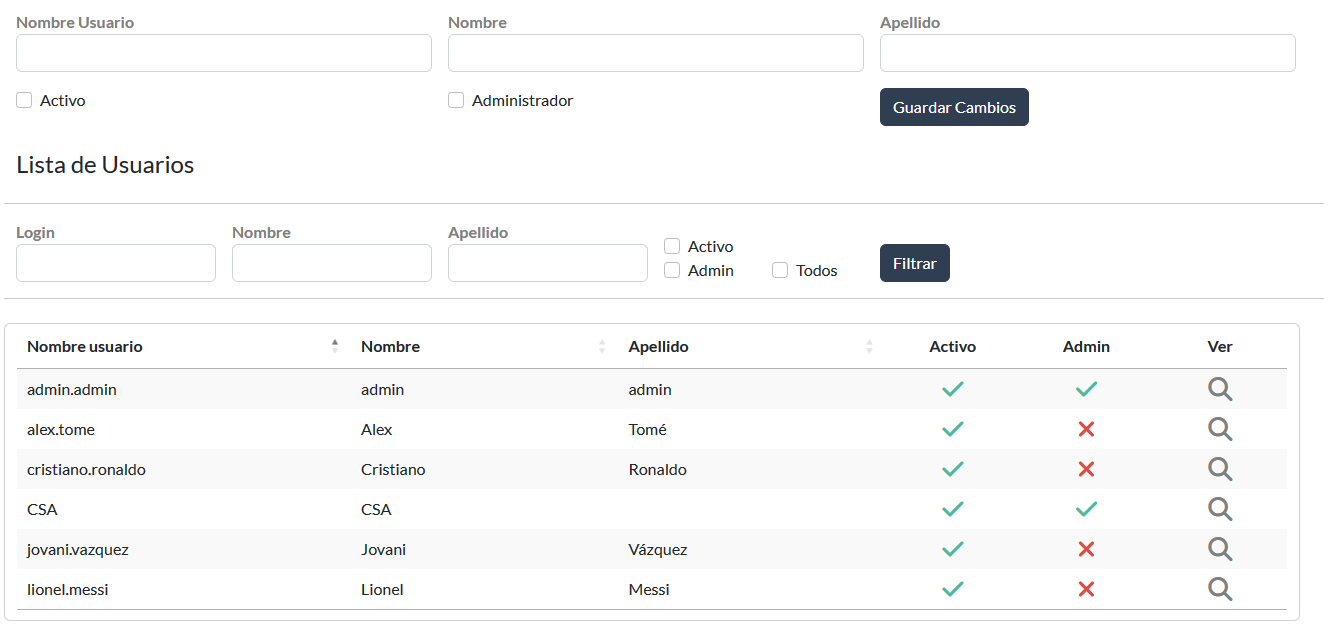
\includegraphics[width=\linewidth]{img/ManualUsuario/Manual18.png}
    \caption{Manual CSACVM - Administración de usuarios}
    \label{manualAU}
\end{figure}

En la parte superior de la figura \ref{manualAU} tenemos los datos del usuario que elijamos a través del botón de ver de la tabla y podremos modificar sus campos. En la parte inferior tenemos la tabla con los usuarios del sistema y un sistema de filtros por los que buscar a los usuarios.






